% \lhead{}
% \rhead{Coulomb's Law}
\newgeometry{left=1in, right=1in, top=1in, bottom=1.2in}

\chapter{Introduction}
This project intends to demonstrate the use of regression techniques to predict housing prices in California. The dataset for the project was downloaded from \href{https://www.kaggle.com/datasets/camnugent/california-housing-prices/data}{www.kaggle.com}. This data was collected during the 1990 census.\\

The project starts with exploratory data analysis (EDA) and data filtering. Then, the variables with the highest correlation with the housing prices were identified. In the next step, linear regression techniques were studied using both single-variable and multi-variable approaches. The multi-variable linear regression performed better than a single-variable linear regression.\\


Furthermore, polynomial regression techniques were explored to model the data. Although the polynomial regression didn't perform on par with the linear regression, the third-degree polynomial was better at predicting the housing prices as compared to the second-degree polynomial.\\

The best predictor was found to be multi-variable linear regression.


\chapter{Data Description}
The data is available as a Comma-Separated Value (CSV) file. The file contains the following items as columns:

\begin{itemize}
    \item \textbf{longitude: }A measure of how far west a house is; a higher value is farther west
    \item \textbf{latitude: }A measure of how far north a house is; a higher value is farther north.
    \item \textbf{housing\_median\_age: }Median age of a house within a block; a lower number is a newer building
    \item \textbf{total\_rooms: }Total number of rooms within a block
    \item \textbf{total\_bedrooms: }Total number of bedrooms within a block
    \item \textbf{population: }Total number of people residing within a block
    \item \textbf{households: }Total number of households, a group of people residing within a home unit, for a block
    \item \textbf{median\_income: }Median income for households within a block of houses (measured in tens of thousands of US Dollars)
    \item \textbf{median\_house\_value: }Median house value for households within a block (measured in US Dollars)
    \item \textbf{ocean\_proximity}Location of the house w.r.t ocean/sea
\end{itemize}
\newpage


\begin{figure}[H]
\centering
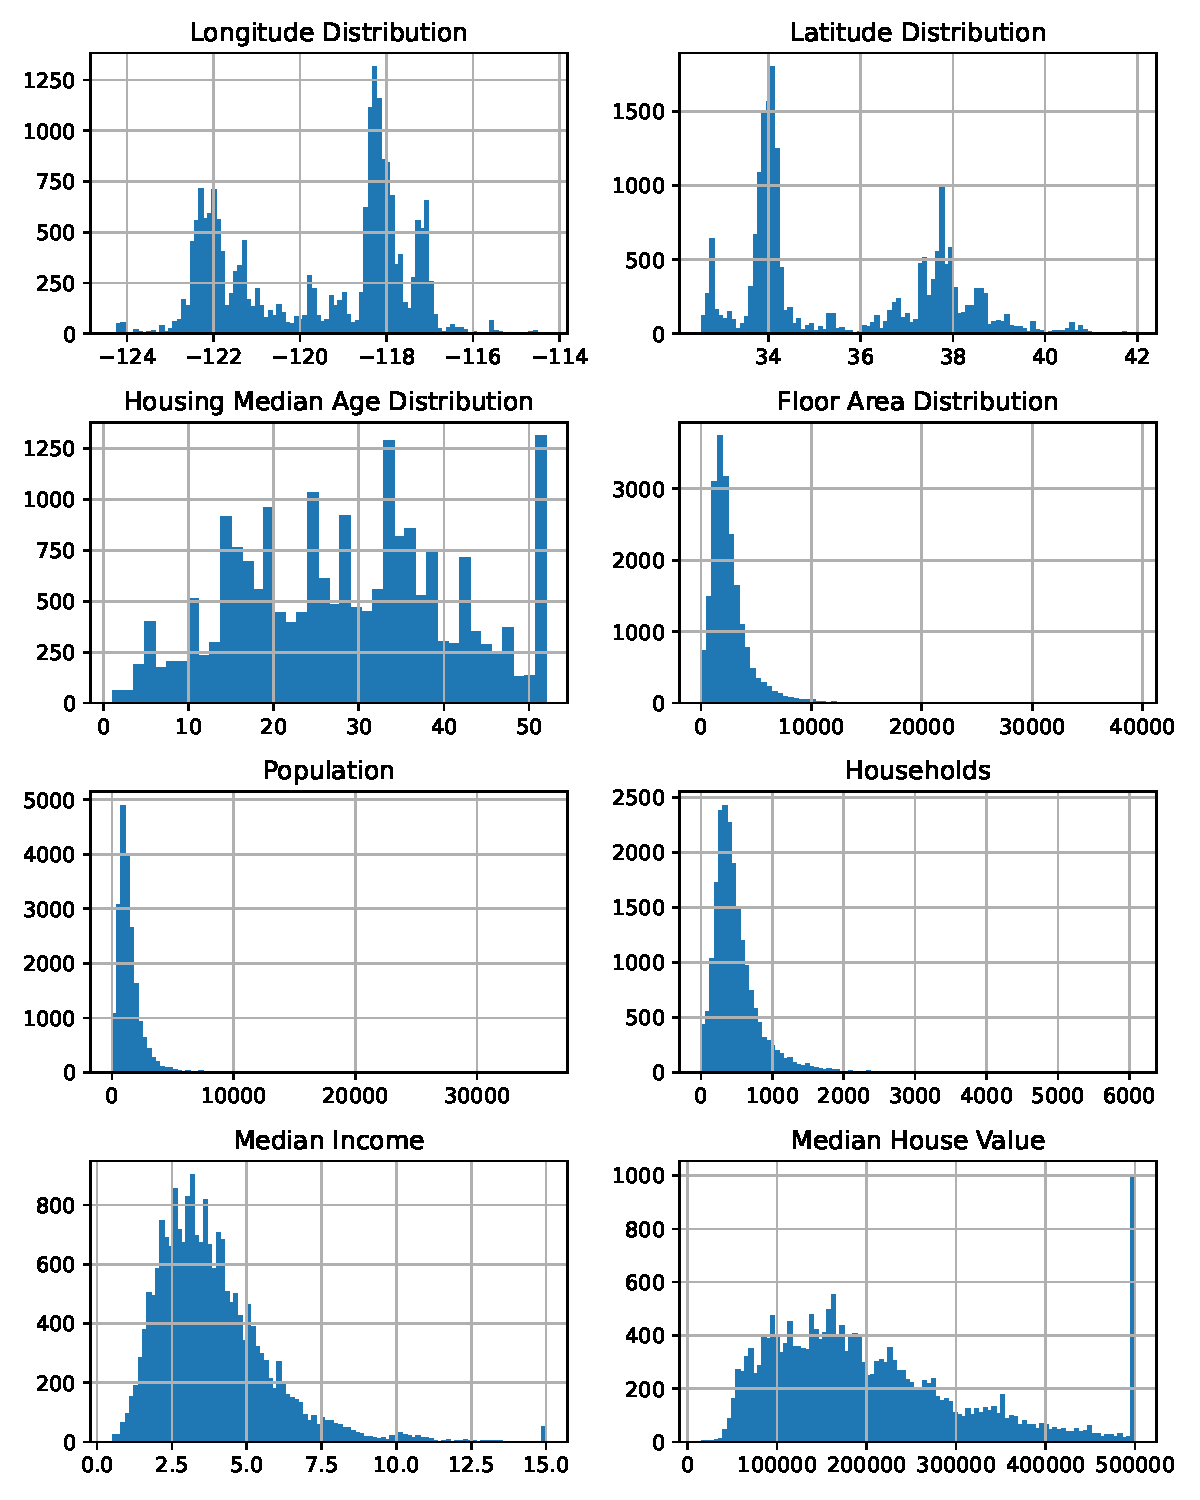
\includegraphics[scale = 0.8]{../figures/housing_distributions.pdf}
\caption{Distributions of variables in the housing dataset.}
\label{fig:housing_distributions}
\end{figure}


The distributions of these variables after cleaning up the null entry rows are summarised in Fig. \ref{fig:housing_distributions}. The latitude and longitude distributions clearly show two strong peaks corresponding to the cities of San Francisco and Los Angeles. The population distribution is fairly Gaussian, while the rest of the distributions are right-skewed Gaussian distributions.\\

The Table \ref{tab:housing_data_summary} outlines a numerical summary of the housing dataset. The dataset contains 20433 rows of non-null entries. 

\begin{table}[H]
\tiny
\begin{tabular}{lrrrrrrrr}
\toprule
 & count & mean & std & min & 25\% & 50\% & 75\% & max \\
\midrule
longitude & 20433.00 & -119.57 & 2.00 & -124.35 & -121.80 & -118.49 & -118.01 & -114.31 \\
latitude & 20433.00 & 35.63 & 2.14 & 32.54 & 33.93 & 34.26 & 37.72 & 41.95 \\
housing\_median\_age & 20433.00 & 28.63 & 12.59 & 1.00 & 18.00 & 29.00 & 37.00 & 52.00 \\
total\_rooms & 20433.00 & 2636.50 & 2185.27 & 2.00 & 1450.00 & 2127.00 & 3143.00 & 39320.00 \\
total\_bedrooms & 20433.00 & 537.87 & 421.39 & 1.00 & 296.00 & 435.00 & 647.00 & 6445.00 \\
population & 20433.00 & 1424.95 & 1133.21 & 3.00 & 787.00 & 1166.00 & 1722.00 & 35682.00 \\
households & 20433.00 & 499.43 & 382.30 & 1.00 & 280.00 & 409.00 & 604.00 & 6082.00 \\
median\_income & 20433.00 & 3.87 & 1.90 & 0.50 & 2.56 & 3.54 & 4.74 & 15.00 \\
median\_house\_value & 20433.00 & 206864.41 & 115435.67 & 14999.00 & 119500.00 & 179700.00 & 264700.00 & 500001.00 \\
\bottomrule
\end{tabular}
\caption{Numerical summary of the housing dataset.}
\label{tab:housing_data_summary}
\end{table}


The aim of the project is to predict housing prices. This requires a study to identify the variables correlated with housing prices. All the variables were compared against the housing price. A graphical summary of the result is given in Fig. \ref{fig:vars_vs_housing_price_distributions}. The latitude and longitude plots show that the median house value depends strongly on location. The cities tend to have more expensive housing, which is also reasonable and expected.\\

The median age of housing and ocean proximity seem to have no correlation with the median house price. In contrast, the total number of rooms, the population in the block, the number of households and the median income seem to have a correlation with the median house value.\\

The median income appears to have the strongest correlation with the median house value.

\begin{figure}[H]
\centering
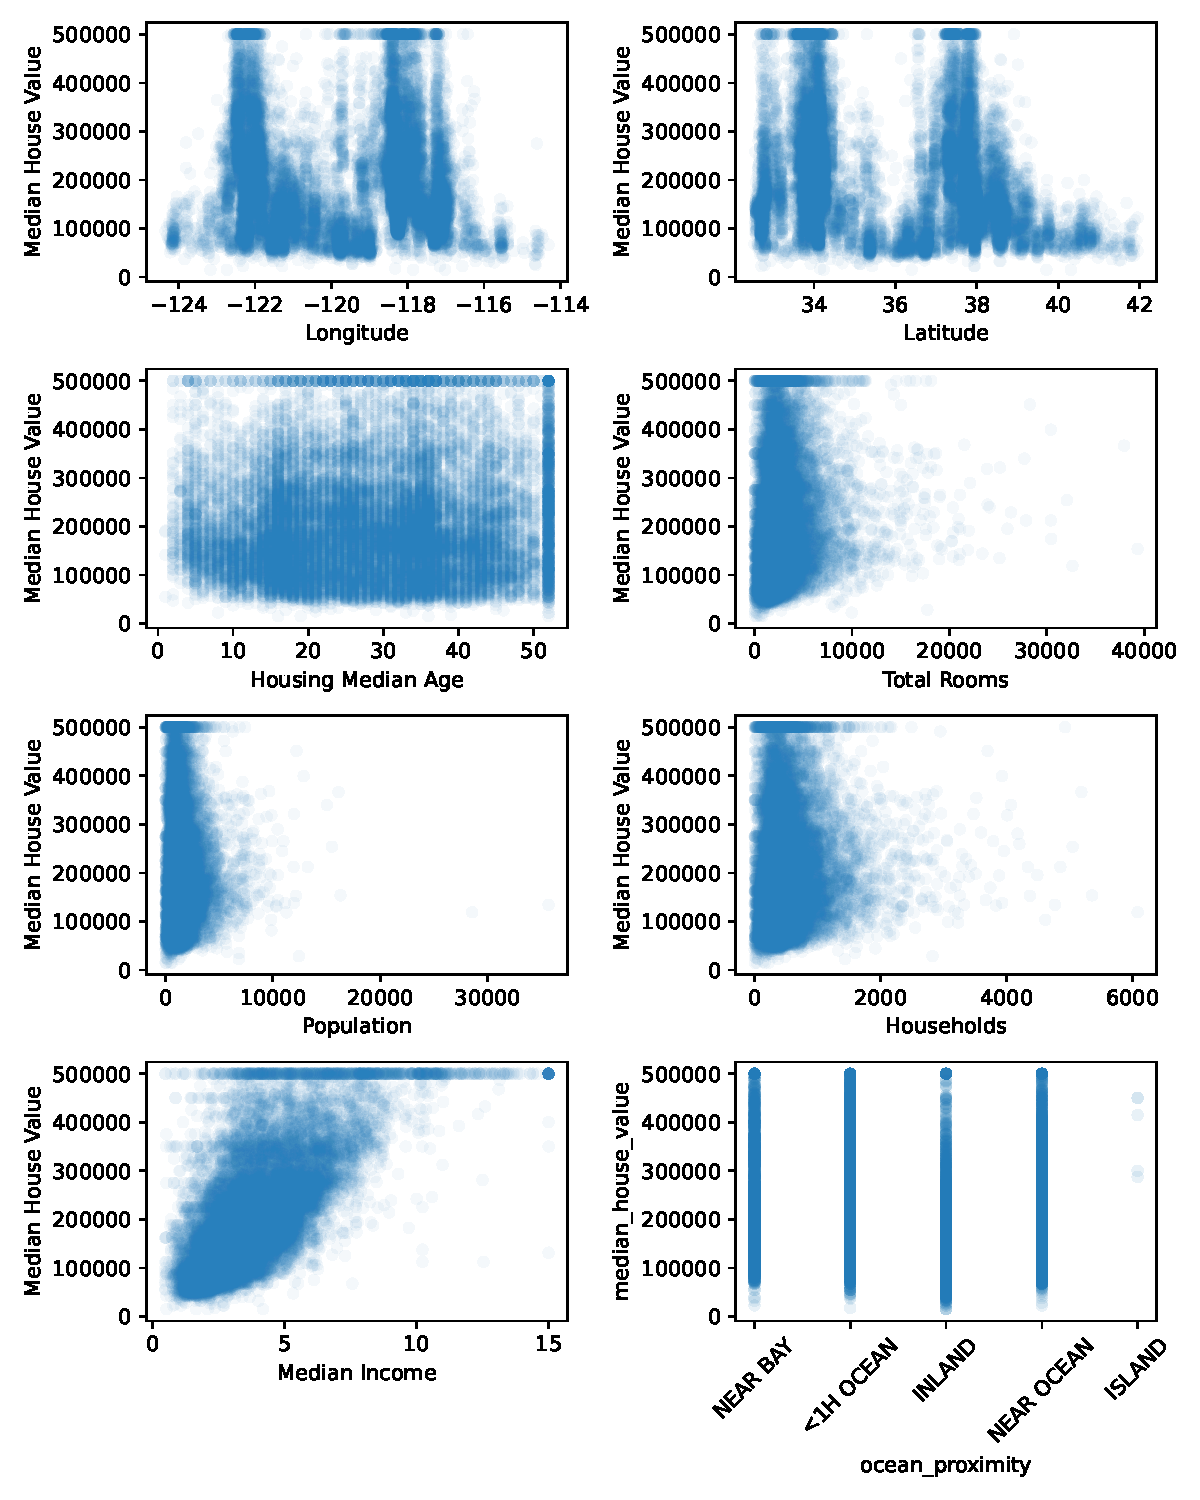
\includegraphics[scale = 0.8]{../figures/median_house_value_vs_variables.pdf}
\caption{Variation of housing price with the various variables in the dataset.}
\label{fig:vars_vs_housing_price_distributions}
\end{figure}


\begin{figure}[H]
\centering

\includegraphics[scale = 0.55]{../figures/variable_correlations.pdf}
\caption{Heatmap of the variable correlations.}
\label{fig:variable_correlations}
\end{figure}

The heatmap shown in Fig. \ref{fig:variable_correlations} shows that median income has highest correlation correlation with the median house value. The other high correlation variables in the order of the magnitude are:

\begin{itemize}
    \item Median Income
    \item Total Rooms
    \item Housing Median Age
\end{itemize}



\chapter{Linear Regression}
Simple Linear Regression with median income as the predictor of the target variable, median house value, was used. The data was split into 80\% and 20\% sets, randomly selected for training and testing, respectively.\\


A summary of the results is shown in Fig. \ref{fig:simple_linear_regression}. The left plot shows the scatter plot of Median Income vs Median House Value. The regression line is shown in red for the test. The regression line seems to describe the correlation nicely. The plot on the right shows the residual i.e. house\_value\_test - house\_value\_test\_predicted. The residual distribution does not show any systematic trend.

\begin{figure}[H]
\centering
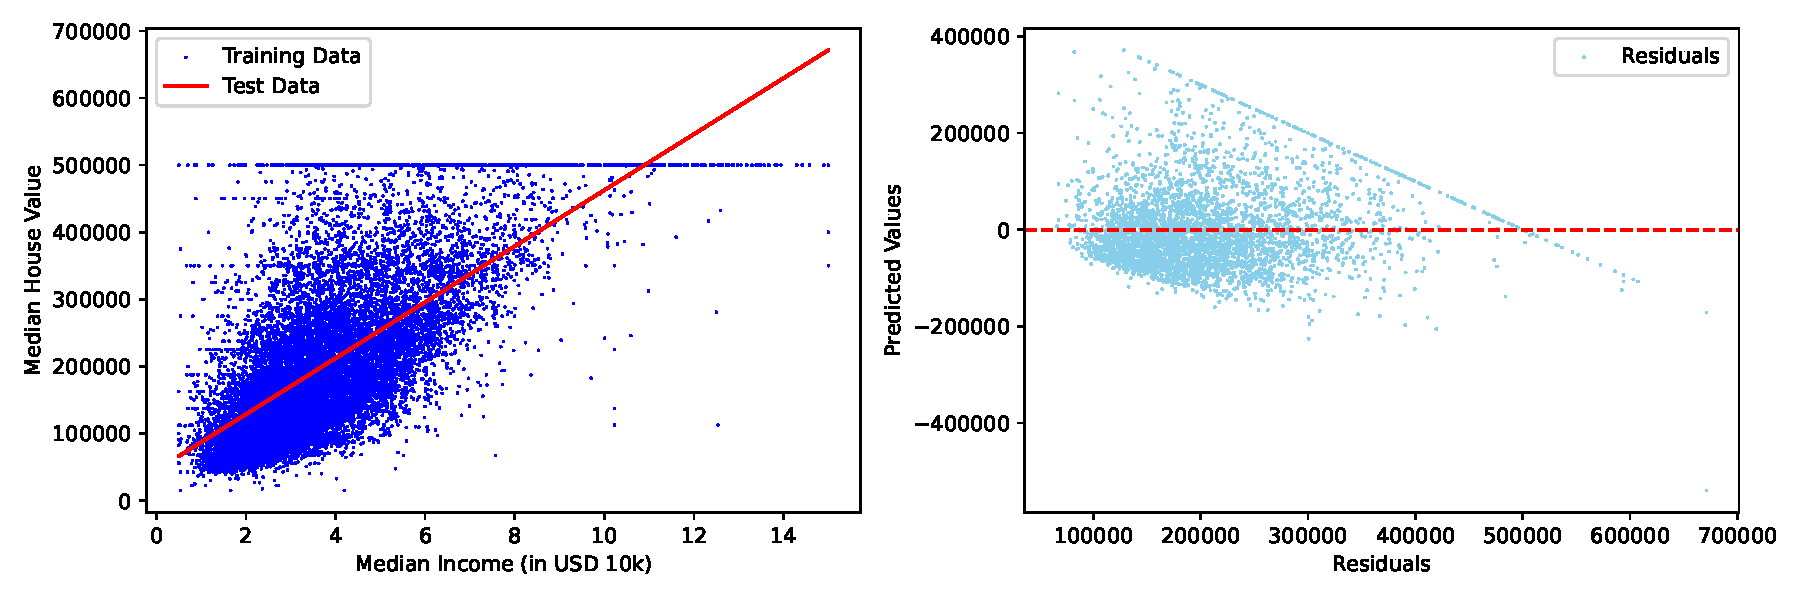
\includegraphics[scale = 0.5]{../figures/baseline_two_variable_regression.pdf}
\caption{Scatter plot of Median Income vs Median House Value on the left and Residual plot on the right.}
\label{fig:simple_linear_regression}
\end{figure}

A numerical summary of the model performance is given below:
\begin{itemize}
    \item The Mean Absolute Error (MAE) was observed to be 62549.25
    \item Root Mean Squared Error (RMSE) was found to be 83638.21
    \item The Coefficient of Determination ($R^{2}$) was observed to be 0.4776.
\end{itemize}

Given the low value of $R^{2}$, a multi-variable linear regression model was explored with the variables most strongly correlated with the median house value, namely median\_income, housing\_median\_age, and total\_rooms. The dataset was split into training and testing sets, and the model was evaluated on the held-out test set. The multi-variable model produced a better fit than the single-variable baseline.\

\begin{figure}[H]
\centering
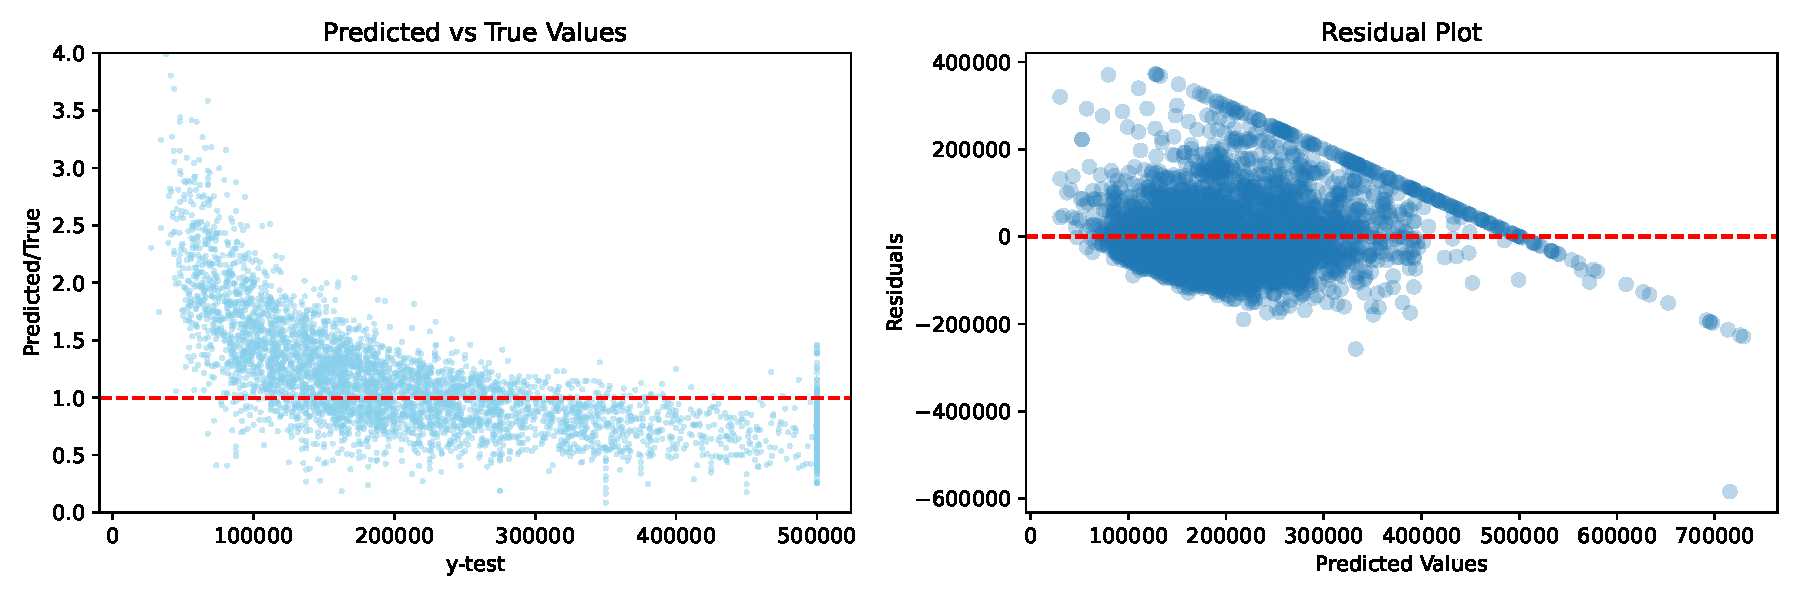
\includegraphics[scale = 0.5]{../figures/baseline_multi_variable_regression.pdf}
\caption{Regression diagnostics for the multi-variable linear regression model.}
\label{fig:multi_variable_regression}
\end{figure}

A numerical summary of the multi-variable regression performance is given below:
\begin{itemize}
    \item The Mean Absolute Error (MAE) was observed to be 60254.02
    \item Root Mean Squared Error (RMSE) was found to be 80511.17
    \item The Coefficient of Determination ($R^{2}$) was observed to be 0.5159.
\end{itemize}

These results indicate that including additional relevant features improves predictive performance, although the model still leaves room for improvement.\

\chapter{Polynomial Regression}
Polynomial regression models were also investigated to test whether nonlinear relationships between median income and house value could improve the predictive accuracy. Two polynomial degrees were considered: second-degree and third-degree.\

\begin{figure}[H]
\centering
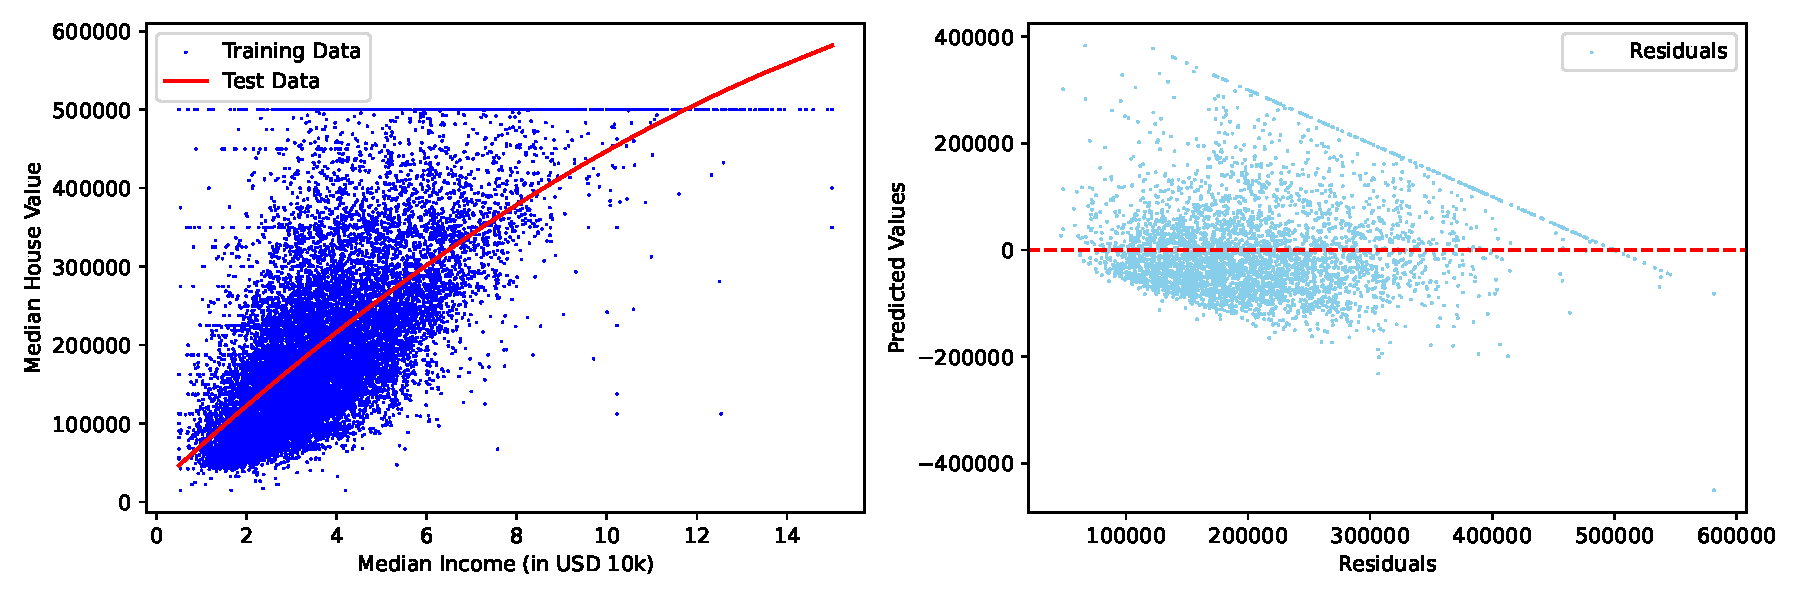
\includegraphics[scale = 0.45]{../figures/second_degree_polynomial_regression.pdf}
\caption{Second-degree polynomial regression fit for median income versus house value.}
\label{fig:second_degree_polynomial}
\end{figure}

The second-degree polynomial model achieved an MAE of 62558.30, an RMSE of 83328.85, and an $R^{2}$ of 0.4814. Although this model slightly improved the fit over the simple linear regression, it still did not outperform the multi-variable linear regression.\

\begin{figure}[H]
\centering
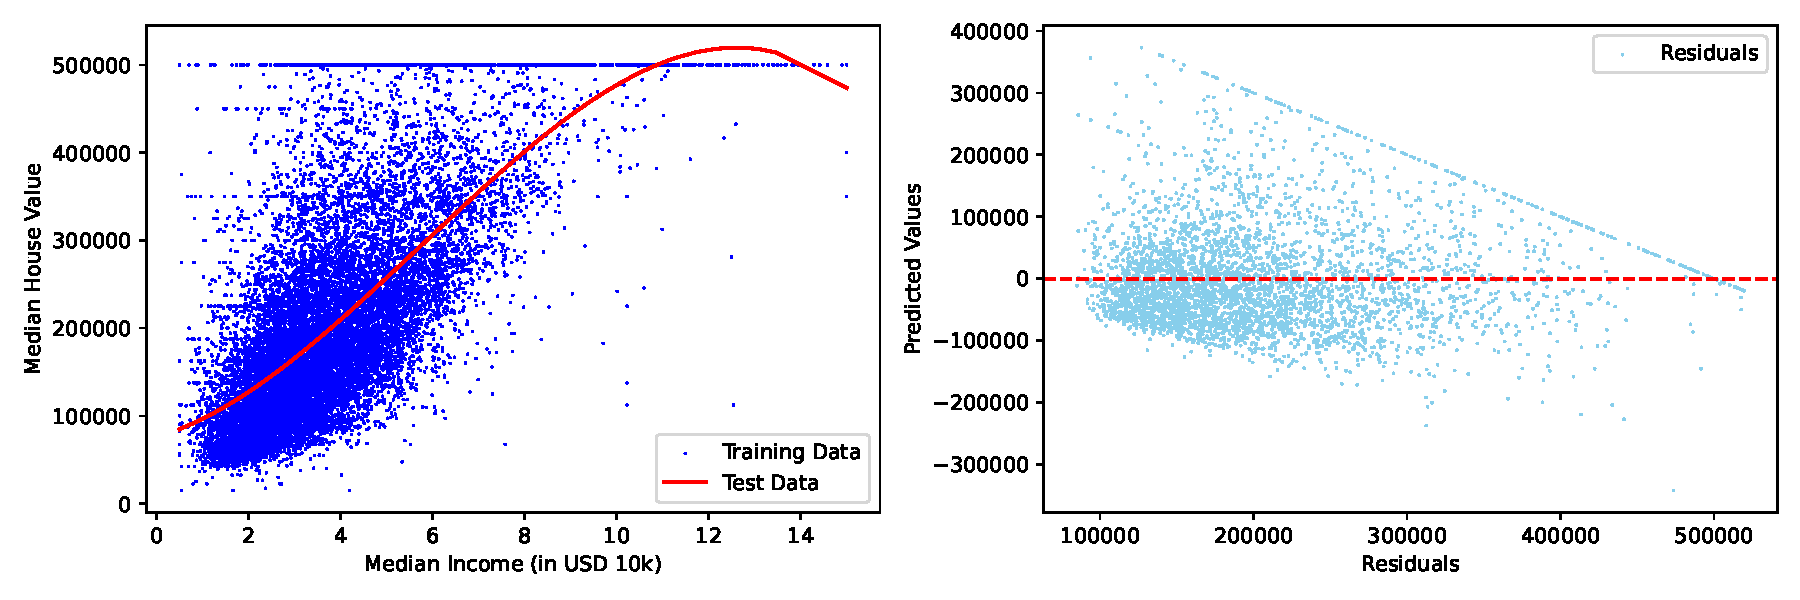
\includegraphics[scale = 0.45]{../figures/third_degree_polynomial_regression.pdf}
\caption{Third-degree polynomial regression fit for median income versus house value.}
\label{fig:third_degree_polynomial}
\end{figure}

The third-degree polynomial model gave a slightly better performance, with an MAE of 61640.86, an RMSE of 82548.27, and an $R^{2}$ of 0.4911. This confirms that the third-degree polynomial performed better than the second-degree variant, but it still remained less accurate than the multi-variable linear regression model.\

Overall, the experiments show that the multi-variable linear regression approach is the strongest model among those tested for this California housing dataset. Future work could explore regularized regression, tree-based models, and additional feature engineering to further improve the prediction quality.

\chapter{Conclusion}
The analysis compared three modeling approaches for predicting California housing prices: simple linear regression, multi-variable linear regression, and polynomial regression. The simple linear regression model, using median income as the only predictor, provided a reasonable baseline but had the weakest performance with a higher MAE and RMSE and a lower $R^{2}$ value. The multi-variable linear regression model improved the predictions by incorporating additional relevant features such as housing median age and total rooms, yielding the best overall performance among all models tested.\

The polynomial regression models were also evaluated, but they did not surpass the multi-variable linear regression. The third-degree polynomial performed slightly better than the second-degree polynomial, yet both remained less accurate than the multi-variable model.\

Overall, the results indicate that the multi-variable linear regression model is the most suitable choice for this dataset because it offers the best balance between interpretability and predictive accuracy. It is therefore the final model recommended for this California housing price prediction task.